\chapter{Solar Oscillation Analysis}\label{chap:solar_osc_analysis}
\epigraph{\textit{Driving out into the Sun\\Let the ultraviolet cover me up\\Looking for a Creation Myth\\Ended up with a pair of black lips}}{\textit{This is the End}\\ \textsc{Phoebe Bridgers}}
Measuring the ``solar'' neutrino oscillation parameters \dmsq{} and \tonetwo{} is one of the principal aims of the SNO+ detector during the scintillator-phase. There are, in fact, two complementary methods of measuring these parameters: the oscillations of anti-neutrinos from terrestrial nuclear reactors, and the oscillations of neutrinos from the Sun.

This chapter focuses on the latter approach, using \beight{} neutrinos coming from the Sun to measure the solar oscillation parameters. An initial background-free study was performed by Javi Caravaca~\cite{caravacaSNOSensitivityStandard2020}, % Javi's tech note
which demonstrated that it was indeed possible to make such a measurement in the detector. The work in this chapter builds on substantially from that analysis. This chapter also draws on the associated reactor anti-neutrino analysis built by Iwan Morton-Blake~\cite{morton-blakeFirstMeasurementReactor2021}, % Iwan's thesis
and more broadly from the general techniques used in the \onbb{} analysis of Tereza Kroupova~\cite{kroupovaImprovingSensitivityNeutrinoless2020} and Jack Dunger~\cite{dungerTopologicalTimeBased2018}.% Tereza & Jack's thesis

This chapter begins by explaining how it is possible to measure the solar oscillation parameters via \beight{} events. Then, the framework used to perform the analysis is then explained: that of a \textit{Bayesian Analysis using Markov Chain Monte Carlo techniques}. After the method has been described, the dataset upon which the analysis is performed is then introduced. The results and associated validation are then given. Given these results, a projection is then made for the expected sensitivity to \tonetwo{} as a function of livetime.


\section{Analysis Methodology}\label{sec:analysis_method}
\subsection{Observational Principle}
How can we measure neutrino oscillation parameters via solar neutrinos in the SNO+ detector? As discussed in Chapter~\ref{chap:theory}, % link to theory section on solar oscillations
it is possible to detect all flavours of neutrino through elastic scattering with electrons in the detector. If this interaction was purely neutral-current, then there would be no way of telling the flavour-state of an interacting neutrino. However, electron neutrinos are able to interact through an additional charged-current mode. This modifies the cross-section for electron neutrinos, and means that as the survival probability for electron neutrinos generated from the Sun, $P_{ee}$, is modified, the interaction probability of neutrinos with the detector will also. The resulting differential interaction rate $R$ for solar neutrinos as a function of the neutrino's energy, $E_{\nu}$, is given by:
\begin{equation}\label{eq:solar_rate}
    \frac{dR}{dE_{\nu}} = 
        \Phi_{\beight{}}S_{\nu}\left(E_{\nu}\right)n_{e}
            \left[
                P_{ee}\left(E_{\nu}\right)\sigma_{\nu_e}\left(E_{\nu}\right) +
                \left(1-P_{ee}\right)\left(E_{\nu}\right)\sigma_{\nu_\mu,\tau}\left(E_{\nu}\right)
            \right],
\end{equation}
where $\Phi_{\beight{}}$ is the total flux of \beight{} solar neutrinos, $S_{\nu}$ is the normalised incident energy spectrum of the solar neutrinos, $n_{e}$ is the number of electron targets in the detector detection medium, and $\sigma_{\nu_{i}}$ is the neutrino-electron elastic scattering cross-section for flavour $i$.

Of course, we do not directly measure neutrino energies in the detector --- only the associated scattered electron. If there were no correlation between the observed electron energy and its associated neutrino, then the only effect of neutrino oscillations would be to change the overall observed rate of events due to this process. There would be no change in the shape of the event's energy spectrum, even though neutrino oscillations are a function of neutrino energy. Fortunately, there is some dependence of $E_{\nu}$ on that of the scattered electron, $E_{e}$. This dependence can be seen in Fig.~\ref{fig:nu_elec_energy_dependence} for \beight{} electron neutrinos interacting in SNO+. % Expected analytical dependence?
As can be seen, the dependence is weak, and comes mostly from basic energy conservation: If one observes a \SI{10}{\MeV} electron event in the detector, it can't reasonably have come from a \SI{5}{\MeV} neutrino.

\begin{figure}
    \centering
    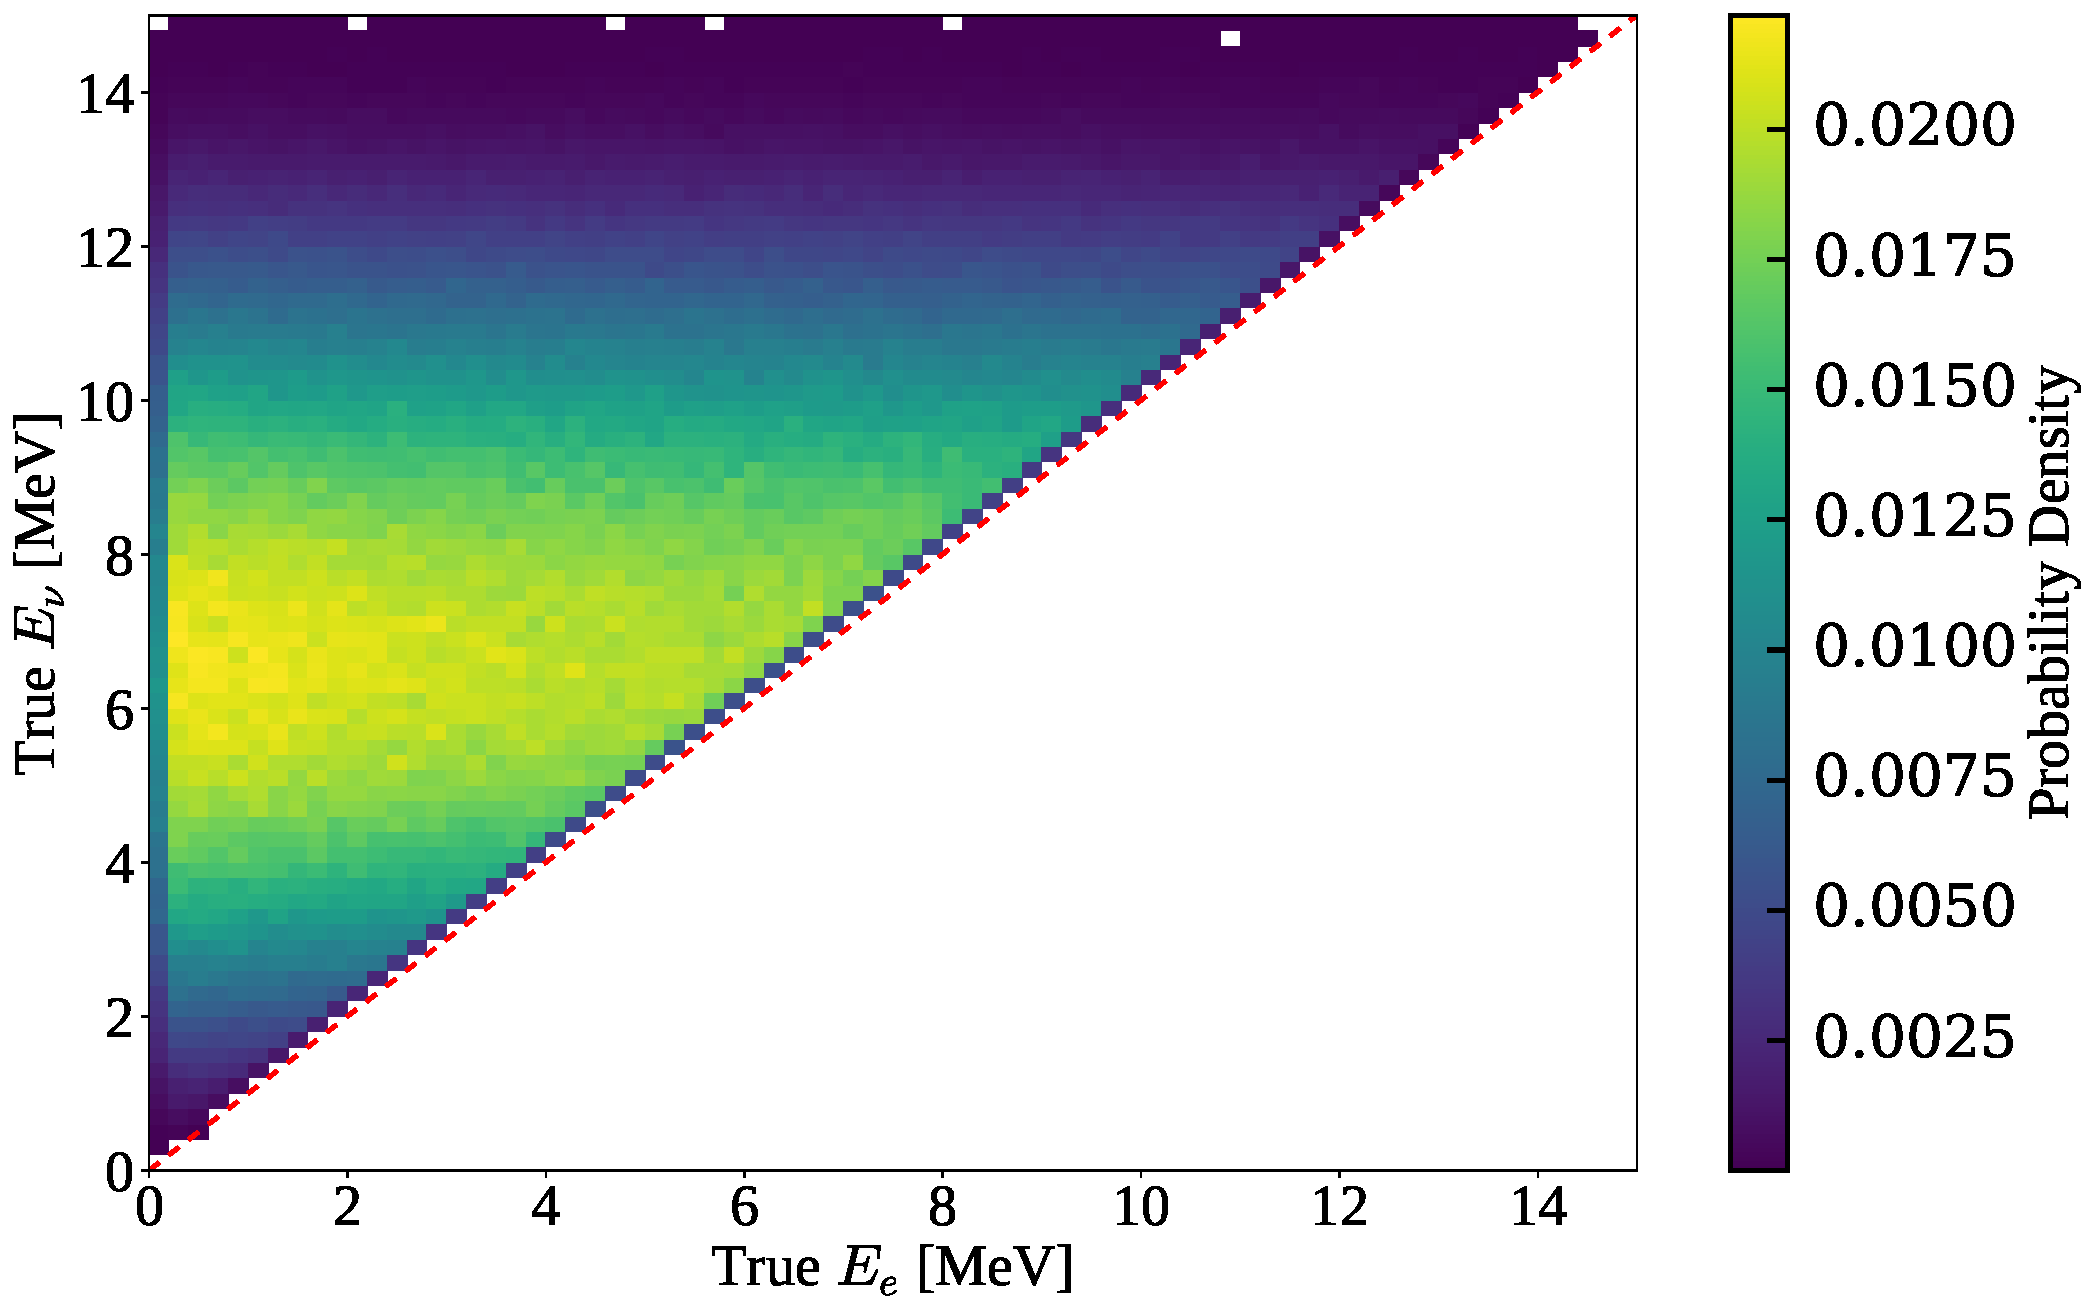
\includegraphics[width=0.8\textwidth]{6_SolarAnalysis/images/b8_eelectrue_vs_enutrue.pdf}
    \caption[True \beight{} $E_{\nu}$ versus true $E_{e}$.]{2D probability distribution comparing the true neutrino energy from a \beight{} $\nu_{e}$ to the true energy of the scattered electron. Also shown in red is the line $E_{\nu} = E_{e}$.}
    \label{fig:nu_elec_energy_dependence}
\end{figure}

\begin{figure}
    \centering
    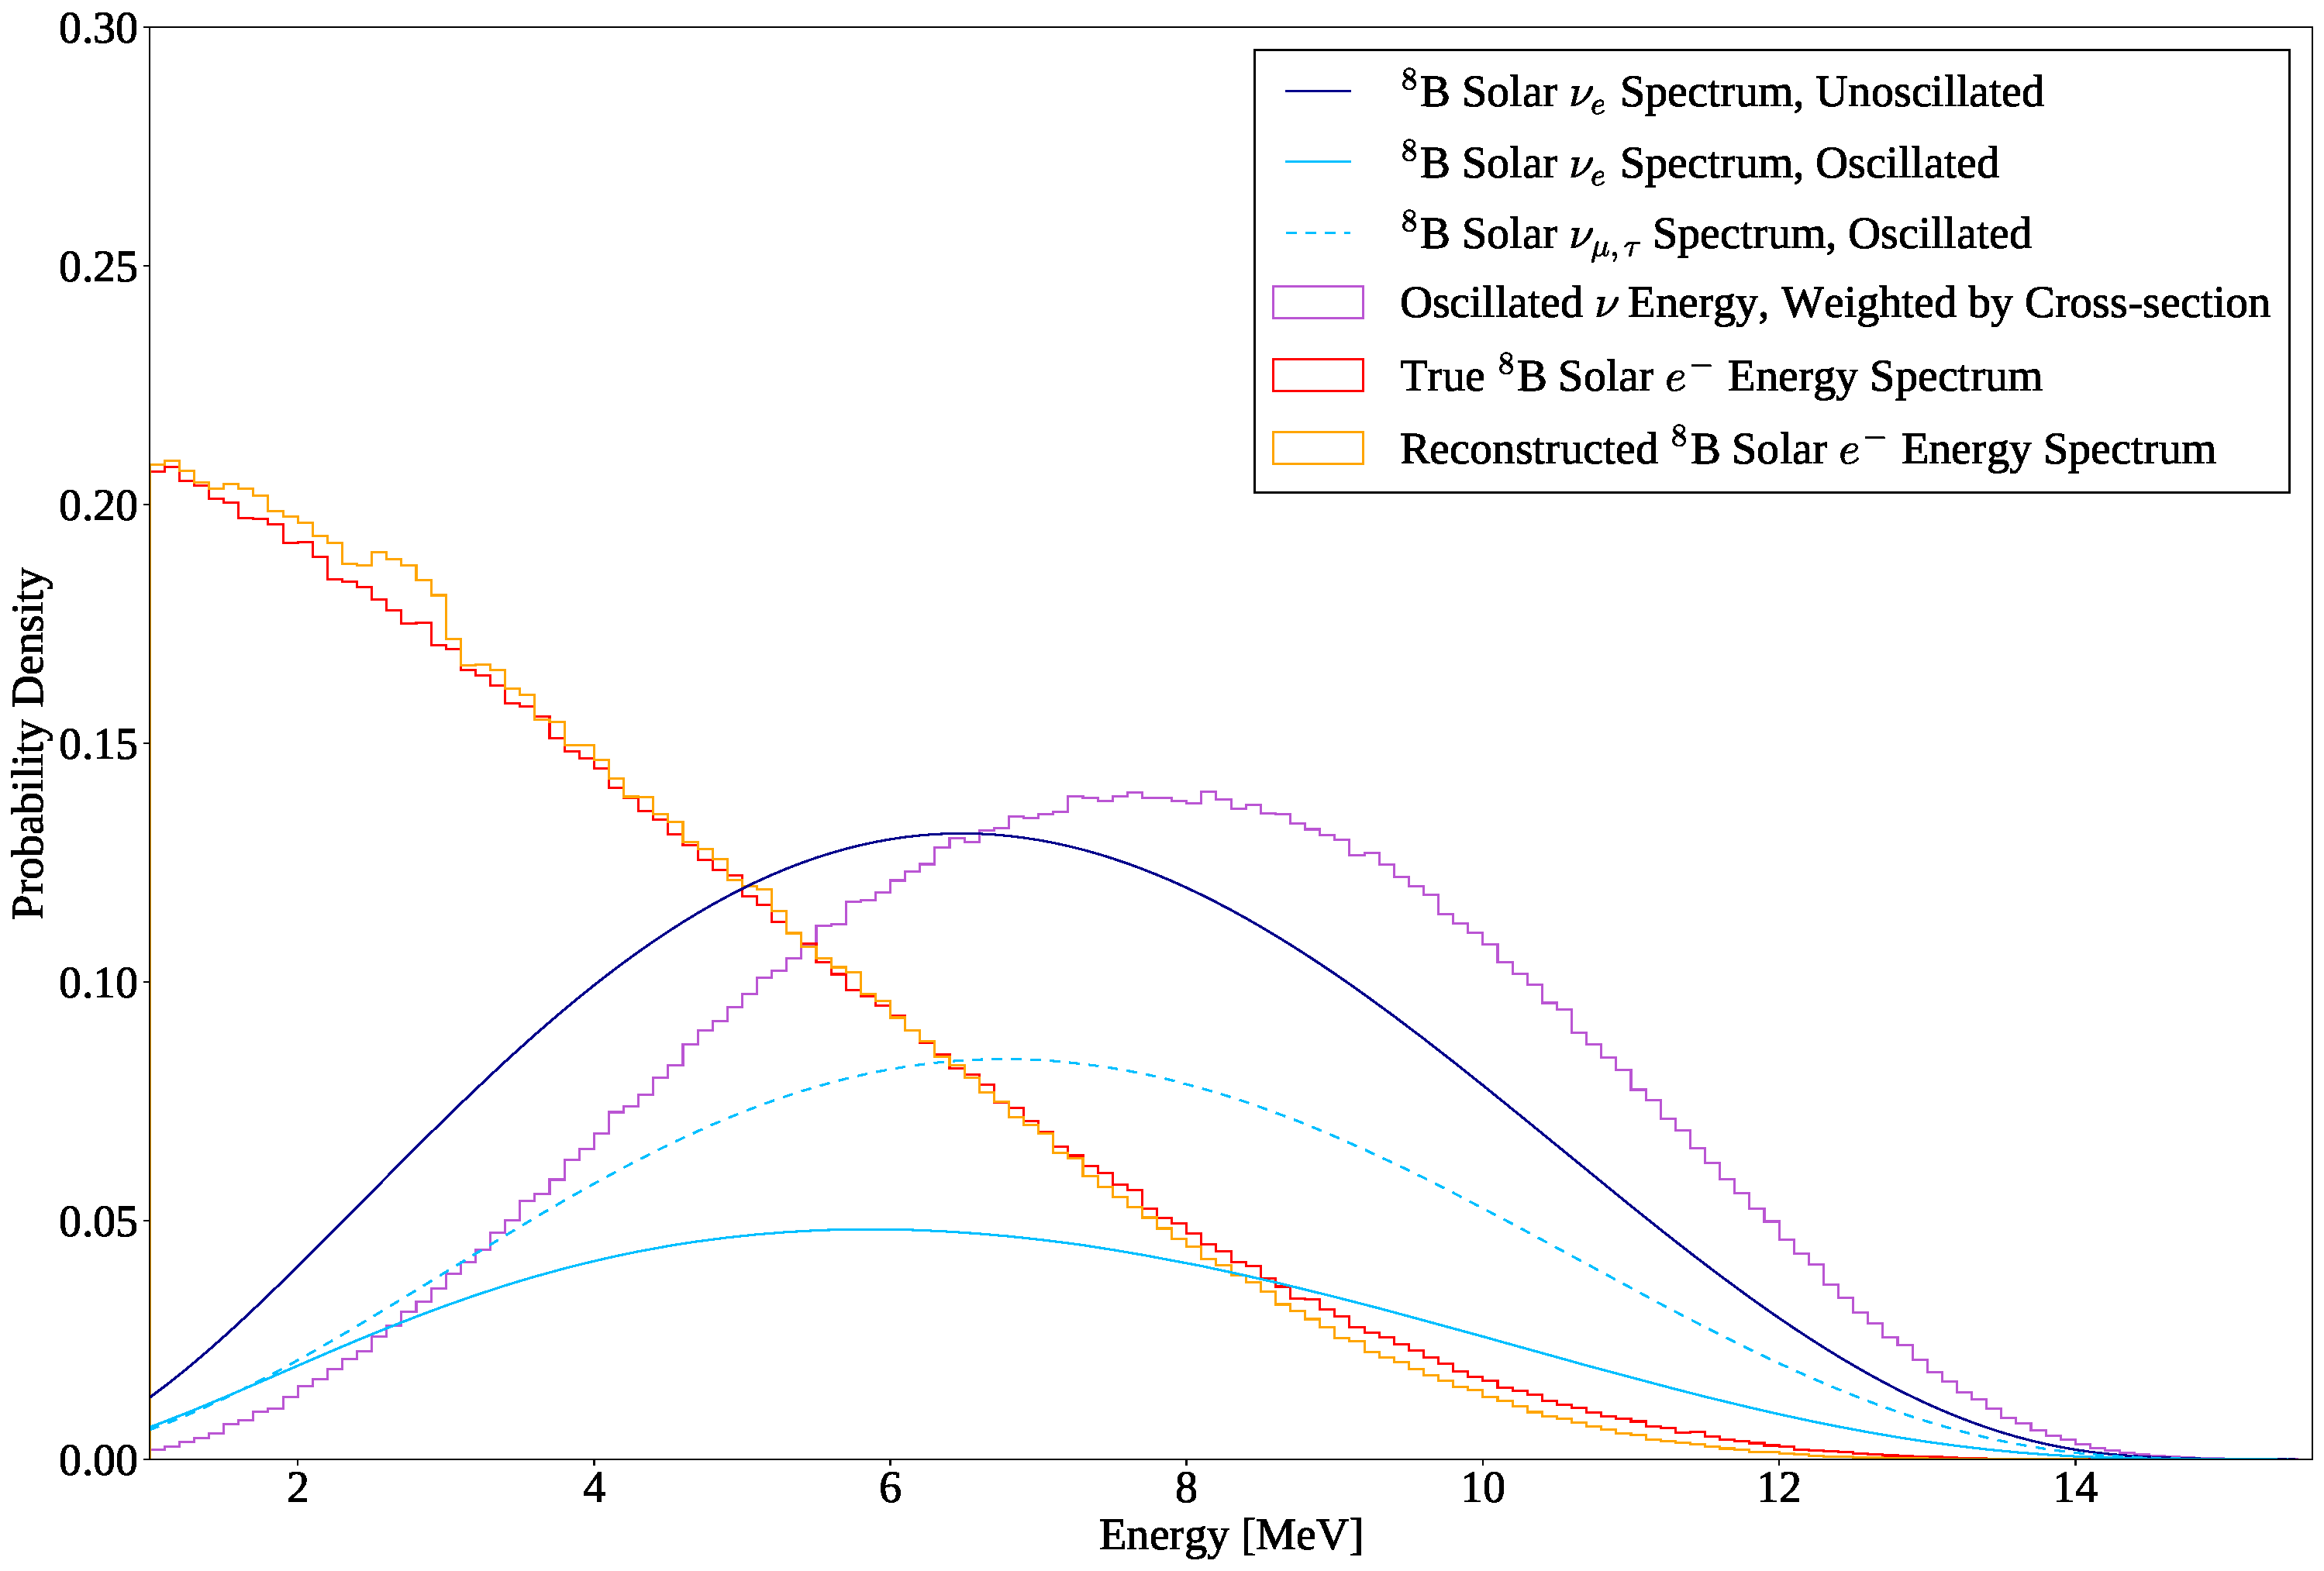
\includegraphics[width=0.75\textwidth]{6_SolarAnalysis/images/b8_energy_evolution.pdf}
    \caption[The evolution of energy distributions related to \beight{} solar neutrino detection.]{The evolution of energy distributions related to \beight{} solar neutrino detection. The unoscillated neutrino spectrum is taken from~\cite{winterB8NeutrinoSpectrum2006}; % cite relevant SSM paper RAT uses
    neutrino oscillations assume oscillation parameters from the current global fit results~\cite{estebanFateHintsUpdated2020} % NuFit
    and $\nu_{e}$ survival probabilities calculated via the method described in Section~\ref{sec:osc_in_fit}. The latter three distributions were obtained from MC production as described in Section~\ref{sec:solar_dataset_livetime}, with the cross-section formula coming from~\cite{bahcallSolarNeutrinosRadiative1995}.% Bahcall radiative corrections paper
    }
    \label{fig:nu_elec_energy_dependence2}
\end{figure}

In Fig.~\ref{fig:nu_elec_energy_dependence2} we can see the impact each physical process has on the energy spectrum that we eventually observe. We start with a broad energy distribution of \beight{} electron neutrinos generated in the Sun. These neutrinos then oscillate their flavour state as they propagate to the detector, in an energy-dependent manner. When a (tiny) fraction of these neutrinos interact with the electrons in our detector, there is both an energy- and flavour-dependence on the cross-section. The scattered electrons gain a kinetic energy with some mild dependence on the inciting neutrino's energy, which is then measured by the detector to within some energy resolution.

Let us now consider the dependence of $P_{ee}$ on the individual neutrino oscillation parameters. Recall from Eq.~\ref{eq:pee_msw} %
that, after considering matter-induced oscillations due to neutrinos passing through the Sun and possibly the Earth, $P_{ee} = P_{ee}\left(\tan2\theta^{M}_{12}, \sin\theta^{M}_{13}, \Delta m^{2}_{21,M}\right) = P_{ee}\left(\theta_{12}, \theta_{13}, \Delta m^{2}_{12}, \Delta m^{2}_{13}\right)$. Fig.~\ref{fig:pee_osc_param_dependence} shows the dependence of each of these four oscillation parameters on $P_{ee}(E)$. We can see that in reality only the two parameters \dmsq{} and \tonetwo{} have a substantial impact on $P_{ee}(E)$ and hence the observed electron energy spectrum. Because of this, for this analysis we will only ever vary these two oscillation parameters, and keep $\theta_{13}$ and $\Delta m^{2}_{13}$ at their current global fit values\footnote{We use the global fit results excluding Super-Kamiokande's atmospheric data, and assuming normal ordering of the neutrino mass hierarchy. This choice has a tiny impact on the magnitudes of these two fixed parameters, the main impact being the sign of $\Delta m^{2}_{13}$.} % Confirm that mass hierarchy has no impact on Pee.
of $\sin^{2}\theta_{13} = 0.0222$ and $\Delta m^{2}_{13} = +\SI{2.515e-3}{\eV\squared}$~\cite{estebanFateHintsUpdated2020}.% nufit citation

\begin{figure}
    \centering
    % \includegraphics[]{}
    \caption[]{}
    \label{fig:pee_osc_param_dependence}
\end{figure}

\subsection{Background Processes}\label{sec:background_processes}
Sadly, elastically-scattered electrons from \beight{} neutrinos are not the only events we see in the SNO+ detector during the scintillator phase. There are a number of background processes that our signal must compete against. Below a reconstructed energy of $\sim\SI{2.5}{\MeV}$, it is known that various backgrounds completely swamp any possible \beight{} signal, and so for this analysis we only consider processes that can generate reconstructed energies of at least $E_{\textrm{min}} = \SI{2.5}{\MeV}$. The following subsections explain each of these backgrounds, as well as methods that have been used to mitigate them as much as possible.

\subsubsection{Internal Uranium- and Thorium-Chain Backgrounds}\label{sec:u_th_internals}
Although every effort has been made to make the scintillator cocktail that fills SNO+ to be as radio-pure as possible, there inevitably remain trace amounts of the radioactive isotopes that derive from the decay chains of the \ce{^{238}U} and \ce{^{232}Th} isotopes. Fig.~\ref{fig:u_th_decay_chains} shows these two decay chains. Fortunately, only a fraction of the radioactive isotopes in these chains actually are capable of generating events in the detector with energies above $E_{\textrm{min}}$: these have been highlighted in Fig.~\ref{fig:u_th_decay_chains} in gold.

\begin{figure}
    \centering
    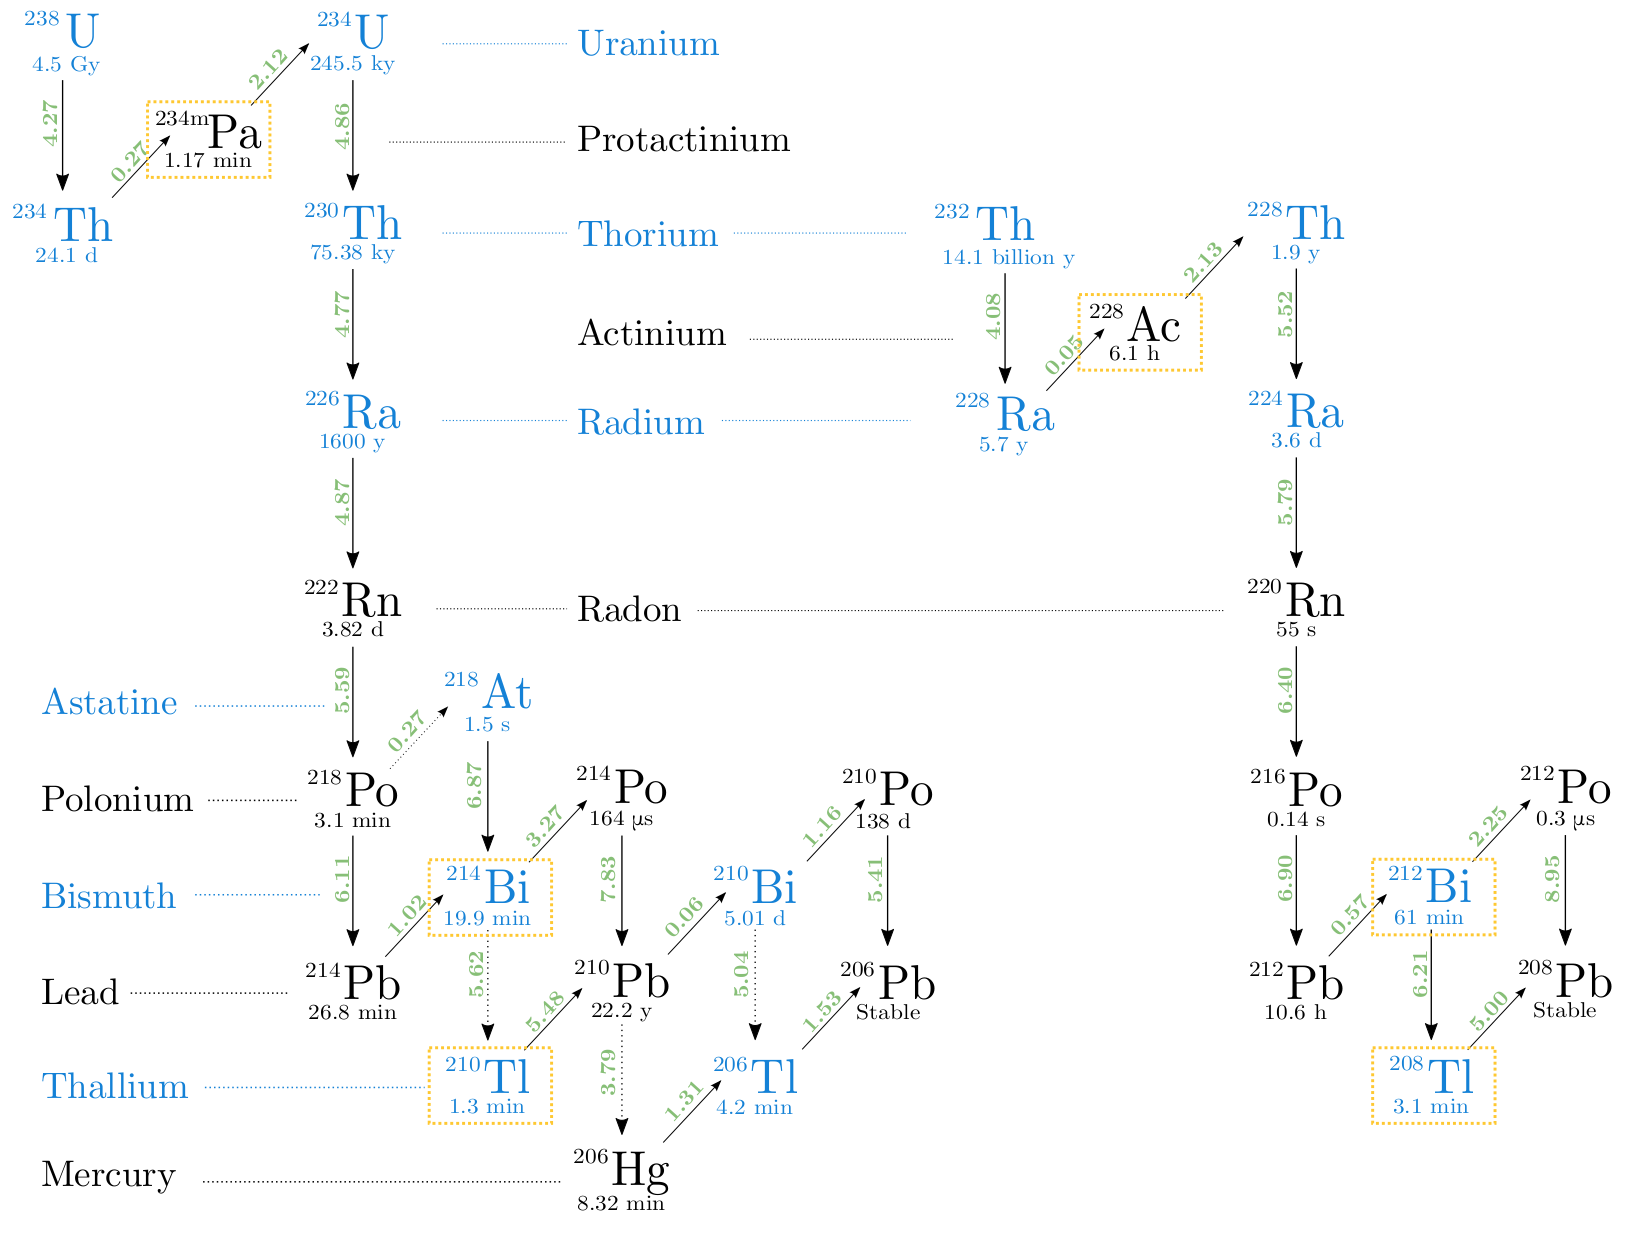
\includegraphics[width=0.75\textwidth]{6_SolarAnalysis/images/U238_Th232_decay_chains_tereza.png}
    \caption[The \ce{^{238}U} and \ce{^{232}Th} decay chains.]{The \ce{^{238}U} and \ce{^{232}Th} decay chains, taken from~\cite{kroupovaImprovingSensitivityNeutrinoless2020}. % Tereza's thesis
    Isotopic half-lives are given below their symbol; the Q-values for each decay, in MeV, is given in green. Downward arrows indicate an $\alpha$-decay; diagonal arrows indicate $\beta$-decay. Isotopes highlighted in gold are potential backgrounds for this solar analysis.}
    \label{fig:u_th_decay_chains}
\end{figure}

Of particular note are the decays of \ce{^{212}Bi} and \ce{^{214}Bi}. Both are capable of either $\alpha\textrm{-}$ or $\beta\textrm{-decays}$ to \ce{Tl} or \ce{Po} isotopes, respectively. For the former, it is the subsequent $\beta$-decay of the \ce{Tl} that can have a reconstructed energy above $E_{\textrm{min}}$. For the latter, the \ce{Bi} decay is the part of the pair of decays that can lie above $E_{\textrm{min}}$. Although the $\alpha$-decays here certainly have Q-values well above \SI{2.5}{\MeV}, the liquid scintillator quenches the observed energy well below $E_{\mathrm{min}}$. The so-called ``\ce{Bi-Po}'' decays are particularly special because the lifetimes of \ce{^{212}Po} and \ce{^{214}Po} are \SI{300}{\nano\second} and \SI{164}{\micro\second}, respectively, which are short enough to allow for highly-effective coincidence tagging.

\nomenclature{\textbf{OOW}}{Out-of-window events}
\nomenclature{\textbf{IW}}{In-window events}
There are two classes of \ce{Bi-Po} event in the detector: ``out-of-window'' (OOW) events for which the \ce{Bi} and \ce{Po} occur in separate event windows, and ``in-window'' (IW) events whereby the \ce{Bi} and \ce{Po} occur within the same event window. These lead to two distinct strategies for tagging these kinds of events. For out-of-window \ce{Bi-Po}s, we look for a delayed coincidence of two events. Using the tagging algorithm suggested in~\cite{} % Jeanne's BiPo tagging DocDB
as a starting point, the chosen procedure was as follows. There must be two events that trigger the detector within \SI{4}{\micro\second} of one another, and both have a valid \texttt{scintFit} position reconstruction within \SI{2}{\metre} of one another. The delayed candidate event must also have at least 100 cleaned PMT hits. %Must ensure cleaned nhits has been explained earlier
This very broad coincidence tagging procedure was designed to ensure that the cut was as \textit{efficient} in tagging (and hence, rejecting) \ce{Bi-Po}s as possible, whilst negligibly impacting the solar signal. This is in contrast to the cuts chosen by Rafael Hunt-Stokes in~\cite{}, % Raf's BiPo tagging tech note on DocDB
which try and obtain a highly \textit{pure} sample of \ce{Bi-Po} tags.

Of course, the above delayed coincidence procedure cannot catch any of the in-window \ce{Bi-Po} events. For these, we use a different approach. Because two decays happened in the same event window, we expect to see two distinct peaks in the event's time residual spectrum. In order to look for this event topology, a likelihood-ratio classifier was run over events, first developed by Eric Marzec~\cite{} % Eric's tech note on DocDB
and re-coordinated for the \SI{2.2}{\gram\per\litre} LABPPO scintillator optics by Ziping Ye~\cite{}. % Ziping's presentation on DocDB
This classifier calculates the likelihood ratio between the null hypothesis of a \onbb{} event (a proxy in this analysis for single-site events such as our \beight{} signal) and the alternative hypothesis of an in-window \ce{Bi-Po} event. The more negative the value of the result, \texttt{alphabeta212}, the greater the evidence there is for rejecting the null hypothesis of a single-site event. Events with $\texttt{alphabeta212} < 0$ % WRITE FINAL CHOICE OF CUT!
were then rejected.

Combining both out-of-window and in-window \ce{Bi-Po} tagging, the impact on \ce{^{212}Bi-Po}, \ce{^{214}Bi-Po}, and \beight{} $\nu_e$ events can be seen in Fig.~\ref{fig:bipo_tagging_efficiency}. We consider here only events that pass all other cuts used in this analysis: see Section~\ref{sec:event_selection} % link to cuts subsection
for the specifics of the cuts used. Because of the different lifetimes of the decays, \ce{^{214}Bi-Po} decays predominantly fall out-of-window whilst \ce{^{212}Bi-Po} events are typically in-window. This explains why the out-of-window tagging is substantially better at cutting \ce{^{214}Bi-Po} decays, whereas the in-window tagging far better tags \ce{^{212}Bi-Po} decays. Overall, within the analysis region of interest (ROI), the two combined cuts are able to tag TODO\% % CALCULATE
of \ce{^{214}Bi-Po} triggered events, TODO\% % CALCULATE
of \ce{^{212}Bi-Po} triggered events, whilst retaining TODO\% % CALCULATE
of \beight{} $\nu_e$ signal events.

\begin{figure}
    \centering
    % \includegraphics[]{}
    \caption[]{}
    \label{fig:bipo_tagging_efficiency}
\end{figure}

\subsubsection{\alphan{} Reactions}
The impact of \ce{^{238}U}- and\ce{^{232}Th}-chain isotopes does not simply end at their direct decays. It is possible for the $\alpha$s generated during these decays to undergo their own interactions with nuclei in the detector. Within the organic scintillator of SNO+, the dominant interaction of this type is when an $\alpha$ collides with a \ce{^{13}C} nucleus, emitting a neutron: \ce{\alpha{} + ^{13}C -> ^{16}O + n}. This is known as an \alphan{} reaction.

The topology of this reaction in the detector is a delayed coincidence, as shown in Fig.~\ref{fig:alpha_n_drawing}. % Iwan's alpha-n sketch
For the prompt signal, there is the light emitted from the $\alpha$ just before, and the \ce{n} just after the \alphan{}. The neutron then thermalises and gets captured by another nucleus --- usually hydrogen in SNO+ --- which creates an excited state that then eventually decays, creating a \ce{\gamma} that creates the delayed signal in the detector~\cite{}. % cite an explanation of alpha-n reactions

\begin{figure}
    \centering
    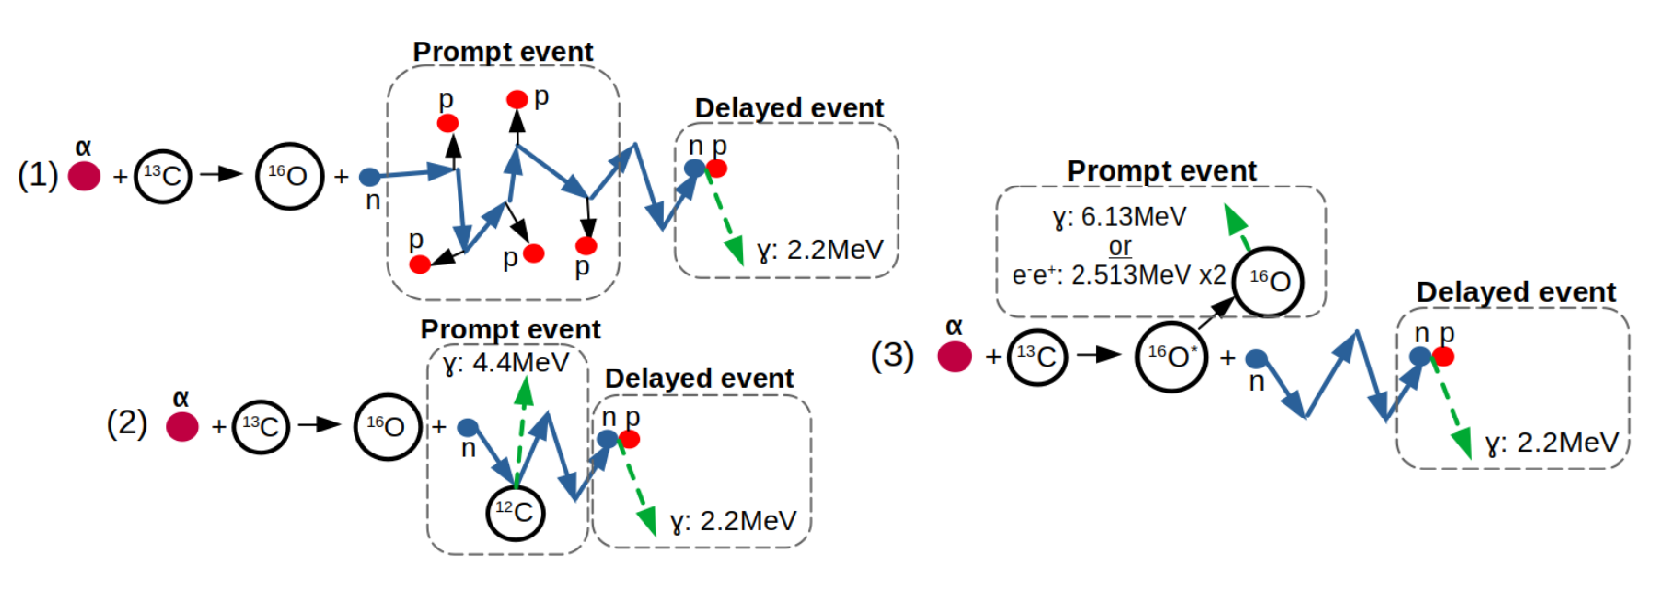
\includegraphics[width=0.8\textwidth]{6_SolarAnalysis/images/alpha_n_schematic_Iwan_modified.pdf}
    \caption[Schematic of \alphan{} interactions.]{Schematic of the three dominant modes of \alphan{} interaction, taken from~\cite{morton-blakeFirstMeasurementReactor2021}. % Iwan's thesis
    }
    \label{fig:alpha_n_drawing}
\end{figure}

As can be seen in Fig.~\ref{fig:alpha_n_coincidence_cut_impact}, \alphan{} interactions can lead to events reconstructed at a wide variety of energies, which could be an issue for this analysis. However, because they are delayed coincidence events with a typical decay time of $\sim\SI{100}{\nano\second}$, the aforementioned out-of-window \ce{Bi-Po} tagging algorithm also efficiently tags \alphan{} events. Looking again at Fig.~\ref{fig:alpha_n_coincidence_cut_impact}, simply by using the out-of-window \ce{Bi-Po} tagger without any further modifications TODO\% of events in the ROI are cut.

\begin{figure}
    \centering
    % \includegraphics[]{}
    \caption[]{}
    \label{fig:alpha_n_coincidence_cut_impact}
\end{figure}


\subsubsection{External Backgrounds}
All materials within the SNO+ detector are radioactive, not just the liquid scintillator cocktail. This includes the acrylic, ropes, external water, and PMTs. These components have had their radiopurity ``assayed'' (that is, measured) throughout the detector's lifetime, often back to the construction of the original SNO detector itself. The materials other than the liquid scintillator are known to have far higher background levels, especially in the important \ce{^{238}U}- and \ce{^{232}Th}-chain backgrounds~\cite{andringaCurrentStatusFuture2016}. % good ref for this
To distinguish between the inherent backgrounds within the scintillator, and the backgrounds from materials at larger radii, we use the terminology ``internal'' and ``external'', respectively.

Although there are numerous external backgrounds, with a suitably accurate and precise position reconstruction algorithm they can be suitably handled. The simplest approach is with a so-called ``fiducial volume'' (FV) cut: just throw out all events that reconstruct beyond some radius. The only external background events that will reach within the FV are those that have reconstructed very poorly, or have some long-distance radiation that manages to deposit radiation close to the centre of the AV. % FOM cut?
Because $\alpha$ and $\beta$ radiation can only travel short distances through the detector, it is only $\gamma$ % and neutron?
radiation that can realistically travel far enough into the detector to be able to reconstruct anywhere near the centre. Moreover, the intensity of this $\gamma$ radiation attenuates exponentially towards the centre of the detector, meaning only a tiny fraction of the total number of external events reconstruct within a \SI{3.5}{\metre} FV, say. This strong radial-dependence can be seen in Fig.~\ref{fig:external_radial_dependence}.

\begin{figure}
    \centering
    % \includegraphics[]{}
    \caption[]{}
    \label{fig:external_radial_dependence}
\end{figure}

What this figure also demonstrates is that our solar signal has a completely different radial dependence to these backgrounds. As a result, if one considers not just the energy of events but also their reconstructed radius, then it is possible to get an additional handle on the external backgrounds. The FV cut can then be pushed further out to larger radii, allowing one to gain more signal statistics.

Work by Tereza Kroupova~\cite{kroupovaImprovingSensitivityNeutrinoless2020} % Tereza's thesis & full-scint re-coordination
allows for additional means of distinguishing external backgrounds from the solar signal. The underlying assumption in the reconstruction of SNO+ events is that there was an electron at a single point, which is entirely valid for \beight{} elastic scattering events. However, external backgrounds can fail this assumption in two ways. Firstly, these radioactive decays often generate $\gamma$ radiation in addition to the main $\alpha$/$\beta$ particle, which creates a multi-site event. Because the \texttt{scintFit} position reconstruction algorithm is not prepared for a distribution of energy depositions in the scintillator, the \tres{} distribution will broaden. This allows an event classifier to be built that distinguishes between the \tres{} distributions of single-site events and externals, known as the ``external background timing classifier''. Secondly, because external backgrounds that do reconstruct close to the centre of the detector typically have a $\gamma$ that travelled a long distance towards the centre of the detector, we expect the earliest light that hits the PMTs to arrive most often along the direction of the reconstructed position vector. A distribution of PMT hits for a given event as a function of their angular distribution relative to the direction of position reconstruction can be built, and compared to the expected distributions for single-site and external background events. This is known as the ``external background topological classifier''. Much like the classifier described in Section~\ref{sec:u_th_internals}, the single-site events used for comparison were \onbb{} events, but these have a similar single-site structure to the solar signal of interest in this analysis.

Fig.~\ref{fig:external_classifier_corr} shows the correlation between the two classifier results for both a typical external background, and \beight{} $\nu_{e}$ events. % DESCRIPTION OF PLOT, HOW A CUT COULD WORK!!

\begin{figure}
    \centering
    % \includegraphics[]{}
    \caption[]{}
    \label{fig:external_classifier_corr}
\end{figure}

\subsubsection{Cosmogenic Isotopes}
The final source of background events are radioactive isotopes that form via collisions of cosmic rays with atomic nuclei, known as cosmogenic isotopes. Most of these isotopes are short-lived~\cite{}, % cite Borexino/KamLAND(?) paper handling cosmogenics
with lifetimes $\mathcal{O}(\SI{1}{\second})$. Fortunately, the depth of SNO+ means that our rate of cosmic ray muons interacting with the detector is only 3 an hour~\cite{}. % cite Lorna/Katharine; Q: confident only muons? What about other kinds of cosmic rays? Presumably nothing else can penetrate this far with high enough rates
Because the rate is so low relative to other experiments, relatively straightforward approaches to tagging and removing cosmic ray muons and their cosmogenic followers can be utilised without substantial loss of livetime. Events are tagged as a cosmic ray muon if they create a sufficient number of hits in the outward-looking PMTs above background levels, as well as many hits within the detector itself. The details of this tagging for the scintillator-fill were put in place by Lorna Nolan~\cite{}, % Lorna's thesis(?); Katharine's contribution?
modifying the existing algorithms used in the water-phase~\cite{} % Billy's Thesis
and in SNO~\cite{}. % Appropriate SNO citation (old thesis?)
After a tagged cosmic muon event, all events for the next \SI{20}{\second} are then vetoed as a means of rejecting followers. This simple cut is enough to remove the vast majority of expected cosmogenic events in the scintillator-phase. % CITATION?
The expected impact on loss of livetime, and hence quantity of signal events, is 3 lots of \SI{20}{\second} vetoes an hour, that is to say 1/60\textsuperscript{th} of the signal is lost via this cut.

There is one cosmogenic isotope with a long-enough half-life that even the \SI{20}{\second} muon follower veto is not sufficient to remove all events. This is \ce{^{11}C}, which \ce{\beta+}-decays to stable \ce{^{11}B} with a half-life of \SI{20.4}{\minute}. The maximum possible energy deposited in this decay is \SI{1.982}{\MeV}~\cite{}, % CITATION
just below $E_{\textrm{min}}$, so only a small fraction of \ce{^{11}C} events end up in the ROI: the ones with very high energies that get their energy reconstruction falsely-inflated by some amount. As a result, this background is expected to be very much sub-dominant to all other backgrounds in this analysis. Because this background is important to consider for some other analyses, a triple-coincidence tagging algorithm is being built by Katharine Dixon~\cite{}, % Katharine C11 citation
but not used for this analysis currently.% Maybe this changes? will see if constraint needed.

\subsection{The Log-likelihood Test Statistic}\label{sec:test_statistic}
At the highest level, this analysis involves taking the data observed in the scintillator-fill after applying a certain set of cuts, along with simulated PDFs for all processes believed to build up the observed data with those same cuts applied, and then attempting to fit the combined energy and radial distributions of the MC to that of the data. Given a set of PDFs, to try and match the distribution of observables in data we can modify a number of parameters. These consist of the normalisations of each PDF (i.e. the total number of events observed due to that process), and any systematic parameters that could modify the shapes of these distributions. For this analysis, the neutrino oscillation parameters act as \textit{de facto} systematic parameters, as they modify the shape of the \beight{} PDFs. Of course, unlike usual systematics the oscillation parameters are what we are actively trying to measure, instead of being a nuisance.

In order to perform a fit to data in this way, we must first answer a set of questions:
\begin{enumerate}
    \item Which signal and background processes must we consider?\label{q:signal_v_background}
    \item In addition to their normalisations, are there any further parameters necessary to specify the distributions of the PDFs for each of the processes? Systematics and oscillation parameters are good examples.
    \item What is our test statistic?\label{q:test_statistic}
    \item What algorithm do we use to try and find the best-fit result?\label{q:algorithm}
    \item How do we measure uncertainties on these best-fit values for each parameter?\label{q:uncertainty}
\end{enumerate}
In section~\ref{sec:background_processes}, question~\ref{q:signal_v_background} was answered for this analysis. We now give the answer to question~\ref{q:test_statistic}; all other questions on this list will be answered shortly.

The test statistic used for this analysis is the \textit{binned extended log-likelihood.} Once the data and MC PDFs have been binned in both the observables of interest, it is assumed that the expected number of events in a given bin $j$ is governed by a Poisson distribution:
\begin{equation}
    P_{j}\left(n_{j} | \lambda_{j}\right) = \frac{\lambda_{j}^{n_{j}}e^{-\lambda_{j}}}{n_{j}!},
\end{equation}
where $P_{j}\left(n_{j} | \lambda_{j}\right)$ is the probability of observing $n_{j}$ events in bin $j$, given an expectation of $\lambda_{j}$ events in total from signal and background processes in that bin. This $\lambda_{j}$ can be decomposed into each of the expected rates for each process, $i$:
\begin{equation}
    \lambda_{j} = \sum_{i=1}^{N_{\textrm{PDFs}}} \mathcal{N}_{i}P_{ij}\left(\bm{\theta}\right),
\end{equation}
where $N_{\textrm{PDF}}$ is the number of PDFs being considered in the analysis, $\mathcal{N}_{i}$ is the normalisation parameter of the $i^{\textrm{th}}$ PDF, and $P_{ij}\left(\bm{\theta}\right)$ is the probability of observing an event of process type $j$ in bin $i$, assuming a set of non-normalisation parameters $\bm{\theta}$. By combining the probabilities of all the bins together, %and also adding the possibility of constraining any of the normalisation or systematic parameters $\bm{\mathcal{N}}$ or $\bm{\theta}$, 
the total probability for a given set of processes assuming these parameters to give rise to the data seen is:
\begin{align}
    P\left(\bm{n} | \bm{\mathcal{N}}, \bm{\theta}\right) = 
    L\left(\bm{\mathcal{N}}, \bm{\theta} | \bm{n}\right) &= 
    \prod_{j=1}^{N_{\textrm{bins}}} \frac{\left[\sum_{i=1}^{N_{\textrm{PDFs}}} \mathcal{N}_{i}P_{ij}\left(\bm{\theta}\right)\right]^{n_{j}}e^{-\sum_{i=1}^{N_{\textrm{PDFs}}} \mathcal{N}_{i}P_{ij}\left(\bm{\theta}\right)}}{n_{j}!},
    % \nonumber\\
    % &\cdot\prod_{k=1}^{N_{\mathcal{N}'}}\frac{e^{-\frac{\left(\mathcal{N}_{k}' - \mathcal{N}_{k}^{\mathrm{nom}}\right)^2}{2(\sigma_{k}^{\mathcal{N}})^{2}}}}{\sqrt{2\pi\sigma_{k}^{\mathcal{N}}}}
    % \cdot\prod_{\ell=1}^{N_{\theta'}}\frac{e^{-\frac{\left(\theta_{\ell}' - \theta_{\ell}^{\mathrm{nom}}\right)^2}{2(\sigma_{\ell}^{\theta})^{2}}}}{\sqrt{2\pi\sigma_{\ell}^{\theta}}}
\end{align}
where $N_{\mathrm{bins}}$ is the total number of bins being considered in the analysis. 
% Gaussian constraints
% \footnote{% note about Bayesian interpretation of constraints
%     As we shall see in section~\ref{}, % reference to Bayesian analysis explanation section
%     because this analysis uses a Bayesian statistical approach, it is more appropriate to talk of these constraints as non-uniform ``priors'' for the parameters.
% } 
% on a subset of the normalisations have been included, $\left\{\mathcal{N}'\right\}$, of which there are $N_{\mathcal{N}'}$ in total. For each of these normalisations, indexed by $k$, there is an associated nominal value $\mathcal{N}_{k}^{\mathrm{nom}}$ and width $\sigma_{k}^{\mathcal{N}}$. There are similar constraints on a subset of the systematic parameters, with similarly-named variables.
This probability can be re-framed as the likelihood of the vectors of parameters $\bm{\mathcal{N}}$ and $\bm{\theta}$ given the vector of number of events in each bin, $\bm{n}$: $L\left(\bm{\mathcal{N}}, \bm{\theta} | \bm{n}\right)$. It is rare to see the likelihood as-is, instead, for computational purposes the log-likelihood is used instead, $\mathcal{L}\left(\bm{\mathcal{N}}, \bm{\theta} | \bm{n}\right) := \ln{L}\left(\bm{\mathcal{N}}, \bm{\theta} | \bm{n}\right)$. We can then get to the formula actually used for this analysis:
\begin{align}
    \mathcal{L}\left(\bm{\mathcal{N}}, \bm{\theta} | \bm{n}\right) &=
    -\sum_{i=1}^{N_{\mathrm{PDFs}}}\mathcal{N}_{i} 
    + \sum_{j=1}^{N_{\mathrm{bins}}}n_{j}\ln{\left(\sum_{i=1}^{N_{\textrm{PDFs}}} \mathcal{N}_{i}P_{ij}\left(\bm{\theta}\right)\right)}.%\nonumber\\
    % &-\sum_{k=1}^{N_{\mathcal{N}'}}\frac{\left(\mathcal{N}_{k}' - \mathcal{N}_{k}^{\mathrm{nom}}\right)^2}{2(\sigma_{k}^{\mathcal{N}})^{2}}
    % -\sum_{\ell=1}^{N_{\theta'}}\frac{\left(\theta_{\ell}' - \theta_{\ell}^{\mathrm{nom}}\right)^2}{2(\sigma_{\ell}^{\theta})^{2}}.
\end{align}


\subsection{The Bayesian Statistical Approach}
There are two main schools of statistical inference, ``Frequentist'' and ``Bayesian''. In the former, probabilities describe the fraction of times a situation can be found within the whole ensemble of possible worlds. For the latter, we care not about an ensemble of worlds but instead our degree of belief in this current one. We update our beliefs as we acquire knowledge of the world through Bayes' Theorem:
\begin{equation}
    P\left(\bm{\mu}|\bm{x}\right) = \frac{\mathcal{L}\left(\bm{\mu}|\bm{x}\right)P\left(\bm{\mu}\right)}{P\left(\bm{x}\right)}.
\end{equation}
Here, $\bm{\mu}$ is the set of parameters that model our system, $P\left(\bm{\mu}\right)$ is our \textit{prior} (pre-existing) distribution for those model parameters, and $\bm{x}$ is the data taken in our experiment. The updated, \textit{posterior} distribution $P\left(\bm{\mu}|\bm{x}\right)$ is then the prior multiplied by the likelihood of parameters $\bm{\mu}$ given observations $\bm{x}$, $L\left(\bm{\mu}|\bm{x}\right)$, and divided by the total probability $P\left(\bm{x}\right)$ of observing $\bm{x}$ under any circumstance.

Both approaches to statistics are widely-used in statistical analysis, in both particle physics and beyond. The Bayesian approach was used for this analysis, as it was believed that this helps keep transparent what assumptions are being made in the analysis. 

Now, if one is able to determine the overall posterior distribution, then it is possible to derive best-fit values with uncertainties for all parameters in the fit. This is done by ``marginalising'' the posterior distribution, i.e. integrating over all parameters other than the one of interest. A sensible best-fit value is then the modal marginalised posterior density, the highest value in the marginalised distribution. The uncertainty on this value is derived from the spread of the marginalised posterior, by the calculation of the $1\sigma$ Credible Interval (CI): this is the set of values for a given parameter which has a total posterior probability of 68.3\%, and contain the best-fit value. There are in fact an infinite number of CIs that satisfy this property; for this analysis, the values are chosen in decreasing order of marginalised posterior probability density.
\subsection{Markov Chain Monte Carlo}
Of course, all of this assumes that one can accurately determine the posterior density distribution. Whilst the likelihood and prior distribution are straightforward enough to calculate, often-times $P\left(\bm{x}\right)$ (which acts as a normalisation) is very challenging to determine. This is because calculating this normalisation involves integrating the likelihood over all the parameter space, and if there are a large number of parameters this can become enormously numerically complex. An alternative approach is needed!

That alternative comes in the form of \textit{Markov Chain Monte Carlo}, MCMC. A Markov Chain is any mathematical system for which the next state of the system is dependent only on its current state; the system is in some sense ``memoryless''. For a large class of Markov Chains --- those that are ``ergodic'' and ``aperiodic'' --- one can prove that regardless of the initial position on the chain, the probability distribution converges to the same distribution~\cite{}. % CITE Feller, W. (1968). An Introduction to Probability Theory and its Applications
MCMC uses such a Markov Chain which attempts to converge towards the posterior density distribution in particular. In MCMC, after choosing the initial position in the parameter space, successive states are chosen at random with a probability dependent only on the properties of the current position in parameter space and the proposed position. The convergence property of Markov Chains means that the set of steps made in the parameter space after some initial number of steps will have a distribution that converges to that of the posterior density distribution.

There are a number of MCMC algorithms, and the particular one used in this analysis is that of the \textit{Random-Walk Metropolis-Hastings Algorithm}. In this algorithm, after the initial position in the parameter space $\bm{\mu}$, a new step is proposed some distance from the current one, $\bm{\mu}'$. This step is chosen at random from a multivariate Gaussian distribution centred on the current position, with widths in each dimension of the parameter space chosen beforehand as constants for tuning the MCMC process. This choosing of a new proposed step at random is what gives the algorithm its Monte Carlo and Random Walk titles. Once a new step is proposed, it is accepted as the new step with a probability $S\left(\bm{\mu}'|\bm{\mu}\right)$ according to the condition of \textit{detailed balance}:
\begin{align}
    S\left(\bm{\mu}'|\bm{\mu}\right) &= 
    \min{\left(
        1,
        \frac{P\left(\bm{\mu}'|\bm{x}\right)}{P\left(\bm{\mu}|\bm{x}\right)}
        \frac{R\left(\bm{\mu}|\bm{\mu}'\right)}{R\left(\bm{\mu}'|\bm{\mu}\right)}
        \right)
        } = 
    \min{\left(
        1,
        \frac{L\left(\bm{\mu}'|\bm{x}\right)P\left(\bm{\mu}'\right)}{L\left(\bm{\mu}|\bm{x}\right)P\left(\bm{\mu}\right)}
        \frac{R\left(\bm{\mu}|\bm{\mu}'\right)}{R\left(\bm{\mu}'|\bm{\mu}\right)}
        \right)
    }\nonumber\\
    &= \min{\left(
        1,
        \frac{R\left(\bm{\mu}|\bm{\mu}'\right)}{R\left(\bm{\mu}'|\bm{\mu}\right)}
        \exp{\left[\mathcal{L}\left(\bm{\mu}'|\bm{x}\right)-\mathcal{L}\left(\bm{\mu}|\bm{x}\right)+\ln{\frac{P\left(\bm{\mu}'\right)}{P\left(\bm{\mu}\right)}}\right]}
        \right)
    }.
\end{align}
$R\left(\bm{\mu}'|\bm{\mu}\right)$ is the probability density that position $\bm{\mu}'$ is proposed as a step from position $\bm{\mu}$, and vice versa for $R\left(\bm{\mu}|\bm{\mu}'\right)$. In most cases, because of the use of the same multivariate Gaussian in choosing proposals, $\frac{R\left(\bm{\mu}|\bm{\mu}'\right)}{R\left(\bm{\mu}'|\bm{\mu}\right)} = 1$ simply. This component only becomes important at the edges of the parameter space, preventing the sampling probability being incorrectly impacted if a proposed step goes outside the allowed parameter space.

It is the detailed balance condition that ensures convergence of the MCMC algorithm to specifically the posterior density distribution. Crucially, because it is only dependent on the ratio of posterior densities, the hard-to-calculate normalisation $P\left(\bm{x}\right)$ in both posterior density terms cancels out, meaning one only needs to calculate the likelihood and priors for each step, as well as $\frac{R\left(\bm{\mu}|\bm{\mu}'\right)}{R\left(\bm{\mu}'|\bm{\mu}\right)}$.

The specific implementation of MCMC used for this analysis is that of \texttt{OXO}, a C++ analysis framework first developed by Jack Dunger~\cite{dungerTopologicalTimeBased2018}. % Jack's thesis
\texttt{OXO} is able to run the Metropolis-Hastings algorithm on multidimensional binned data, using the log-likelihood defined in~\ref{sec:test_statistic}. This framework also allows one to include systematic parameters that can float within the fit, and define non-uniform priors for normalisations and systematics that have constraints: the details of this will be discussed shortly.

\subsection{Choosing Priors}
For this analysis, the suggestions made by Biller \& Oser in~\cite{billerAnotherLookConfidence2015} % Steve's stats paper 
about choosing prior distributions are followed: for parameters that do not have some pre-existing constraint, a flat prior is used. A nice consequence of this choice is that $\ln{\frac{P\left(\bm{\mu}'\right)}{P\left(\bm{\mu}\right)}} = 0$, so the actual value of the prior for these variables never needs to be calculated when running the MCMC algorithm. For the bulk of this analysis, uniform priors are assumed on the neutrino oscillation parameters \dmsq{} and \tonetwo{}, as the magnitudes of these parameters are now well-established.

For parameters with existing asymmetric constraints $\beta^{+\sigma_{+}}_{-\sigma_{-}}$, this analysis uses an asymmetric Gaussian prior, equivalent to the logarithm of the prior being an asymmetric quadratic:
\begin{equation}
    \ln{P\left(\mu\right)} = \mathcal{A} -
    \begin{cases}
        \frac{\left(\mu-\beta\right)^{2}}{2\sigma_{+}^{2}} & \textrm{if } \mu\geq\beta,\\
        \frac{\left(\mu-\beta\right)^{2}}{2\sigma_{-}^{2}} & \textrm{if } \mu<\beta.
    \end{cases}
\end{equation}
Here, $\mathcal{A}$ is the logarithm of the prior's normalisation constant, and cancels out in the detailed balance condition. For parameters with symmetric constraints, $\sigma_{+}=\sigma_{-}$, then $\ln{P\left(\mu\right)}$ reduces to a quadratic with maximum at $\mu = \beta$.

\subsection{Including Systematics in the Fit}
One important implementation detail is how systematics are applied within the MCMC fitting process. Once systematics are added to the fit, at every step the binned PDFs for all the processes considered in the fit must get modified appropriately, which can become extremely computationally-intensive if not approached carefully. The strategy used in the \texttt{OXO} framework starts by thinking of the contents of a binned PDF as a vector of bin probabilities, $\bm{\mathrm{p}} = \left(p_{1}, p_{2}, ..., p_{N_{\textrm{bins}}}\right)^{T}$. Then, we can think of a systematic acting on the PDF as a linear transformation, and hence a matrix $S$ acting on this vector: $\bm{\mathrm{p}'} = S\bm{\mathrm{p}}$. We only need to calculate this matrix once for a given set of systematic parameter values, and can then use the same matrix on all the PDFs in the fit. Furthermore, when multiple systematics are applied, the matrix for each systematic can then be combined via matrix multiplication into one single ``detector response'' matrix. \texttt{OXO} uses the \texttt{Armadillo}~\cite{} % Armadillo software citation
linear algebra package for efficient matrix manipulation.

There is a problem that can arise when considering the impact of systematics near the edge of the analysis ROI. Many systematics such as shifts, scalings, and convolutions use information about the contents of nearby bins to determine the contents of a particular bin. However, for bins near the edge some of that information does not exist --- it has been lost to the cuts that define the ROI. This can lead to a bias in the generation of the modified PDFs, and therefore also the posterior distribution.

As an example, consider the impact of an energy scale systematic on the energy distribution of \ce{^{234m}Pa} events in the detector, shown in Fig.~\ref{fig:energy_scaling_example}. Because the events seen for this process in the ROI are merely the high-energy tail, any systematic energy scaling $E'_{\textrm{reco}} := \beta E_{\textrm{reco}}$ should have a large impact on the number of events observed at the low end of the ROI. However, given that the information about data below $E_{\textrm{min}}$ is lost to the ROI cuts, any energy scaling of $\beta>1$ will not be applied correctly at all.

\begin{figure}
    \centering
    % \includegraphics[]{}
    \caption[]{}
    \label{fig:energy_scaling_example}
\end{figure}

The solution to this problem is defining a ``buffer region'' of bins on either side of the ROI, which allow for tracking of events in and out of the ROI due to systematics, but aren't considered when calculating the likelihood. This is also shown in Fig.~\ref{fig:energy_scaling_example}. After the scaling systematic is applied, although incorrect bin values are found in the buffer region, this is fine because we are no longer calculating the likelihood with those bins. Note that because of this modification, the normalisation parameters we put into the model no longer represent the expected number of events in the ROI. Instead, they represent the number of events expected in both the ROI and buffer region, before any systematics have been applied.


\subsection{Including Oscillations in the Fit}\label{sec:osc_in_fit}
Within the analysis MCMC code, the process of neutrino oscillations are thought of as a \textit{de facto} systematic that acts only on the \beight{} $\nu_{e}$ and $\nu_{x}$ signal spectra. Three parameters relevant to the signal are floated within the MCMC fit: \dmsq{}, \tonetwo{}, and $\Phi_{\ce{^{8}B}}$, the unoscillated \ce{^{8}B} flux relative to the expected rate. For the two signal PDFs, a third ``bookkeeping'' dimension is added on top of reconstructed energy and radius: the true neutrino energy, $E_{\nu}$. This is necessary for correctly applying oscillations, as the oscillation probability is a function of the neutrino's energy, not the scattered electron's. Before the fit, these 3D PDFs are given normalisations corresponding to the expectation of the number of events for each type, $\nu_{e}$ and $\nu_{x}$, after cuts but before oscillations have been applied. Strictly speaking there should be zero $\nu_{x}$ events before neutrino oscillations: the pre-oscillation rate used here is the post-cut number of events expected if 100\% of the neutrinos oscillated to the $\nu_{x}$ type.

During the MCMC fit, for a given set of parameters $\bm{\theta} = \left(\dmsq{}, \tonetwo{}, \Phi_{\ce{^{8}B}}\right)$ the following is performed to oscillate the signal PDFs. Firstly, the normalisations are scaled by the factor $\Phi_{\ce{^{8}B}}$. Then, for each $E_{\nu}$ bin the survival probability $P_{ee}\left(E_{\nu}, \dmsq{}, \tonetwo{}\right)$ is calculated. Each bin then has their probability scaled by either $P_{ee}$ or $1-P_{ee}$, for $\nu_{e}$ and $\nu_{x}$ respectively. Of course, within the structure of the \texttt{OXO} framework these bin-by-bin scaling aren't immediately applied, but instead a matrix describing the impact of oscillations on each of the PDFs is made. Because the oscillation transformation is purely a bin-by-bin scaling, the resulting matrices are diagonal, with diagonal elements $\Phi_{\ce{^{8}B}}\cdot P_{ee}\left(E_{\nu}, \dmsq{}, \tonetwo{}\right)$ or $\Phi_{\ce{^{8}B}}\cdot\left(1-P_{ee}\left(E_{\nu}, \dmsq{}, \tonetwo{}\right)\right)$ for $\nu_{e}$ and $\nu_{x}$ respectively. After the oscillation matrix along with all other systematic matrices are applied to the signal PDFs, the PDFs are then marginalised over the $E_{\nu}$ dimension so that the signal PDFs match the dimensionality of all other processes.

Calculations of the survival probability are handled with \texttt{PSelmaa}, an algorithm written by Nuno Barros for the SNO 3-phase Analysis~\cite{}. % Nuno's thesis
This considers not only the neutrino oscillations through the vacuum of space between the Sun and Earth, but also the impact of matter effects in both the Sun and Earth. This can usually be a very computationally-intensive process, but \texttt{PSelmaa} takes advantage of the assumption that the solar oscillation parameters are in the so-called ``Large Mixing Angle'' regime, making the calculation much faster. As seen in Section~\ref{sec:nu_osc_evidence}, % ref chapter 1
previous solar oscillation experiments demonstrate that this assumption is reasonable. For this analysis, the standard MSW effect is assumed with neutrinos obeying the Normal Hierarchy, with the Sun following the \texttt{B16\_GS98} metallicity model~\cite{} % CITE
and the \texttt{PREM} model being used for the Earth~\cite{}. % CITE
% Discussion of why these models and not others?

One final thing \texttt{PSelmaa} needs to know to calculate survival probabilities is the distribution of solar zenith angles during the data-taking. The solar zenith $\theta_{z}$ is the angle between the two following vectors: one going from the centre of the Earth through the centre of the SNO+ detector, and another starting from the detector's centre and pointing towards the Sun. As an example, if the Sun were ever to be directly overhead the detector, both vectors would be along direction $\bm{\hat{z}}$ in detector coordinates, leading to a solar zenith angle of $\theta_{z}=0$. The position of the SNO+ detector on Earth, as well as the times at which the detector was live, determine the solar zenith angle distribution. If not accounted for, this can lead to a bias in the result of the analysis, as a preponderance of livetime taken at night (say) would lead to a larger fraction of solar neutrinos having to pass through the bulk of the Earth to get to the detector, and hence the impact of the MSW effect would be greater.

Even after using the Large Mixing Angle approximation, having to call \texttt{PSelmaa} numerous times for every step in the MCMC algorithm would lead to exorbitant run times for the fitting. Therefore, a further approximation is made. Before running the MCMC fit, \texttt{PSelmaa} is used to calculate $P_{ee}$ over the necessary 3D space of parameters. To get a fine scan of this space, 101 $E_{\nu}$ values from \SI{1}{\MeV} to \SI{20}{\MeV}, 101 \dmsq{} values from \SI{3e-6}{\eV\squared} to \SI{1e-3}{\eV\squared}, and 151 values for \tonetwo{} from \ang{5} to \ang{65} were looked over. This 3D grid of $101\cdot101\cdot151$ $P_{ee}$ values is then written to disk, and loaded into memory for use during the fit as a lookup table. At run-time, as the Metropolis-Hastings algorithm samples this 3D space the survival probability is estimated through a trilinear interpolation of the 3D grid loaded in: a version of linear interpolation for three dimensions~\cite{}. % trilinear interpolation citation
% Discussion of minor systematic associated with linear interpolation?

    %  \begin{itemize}
        % \item Start with observational principle: changes in oscillation parameters lead to change in the energy spectrum of neutrinos elastically-scattering in the detector, and hence a change in the observed energy spectra of elastically-scattered electrons within the detector. Demonstrate basic impact on modifying $\Delta m^{2}_{21}$ and $\theta_{12}$.
        % \item Want to maximise the sensitivity to measuring these two parameters. Energy spectrum of signal is background-free above $\sim\SI{5}{\MeV}$, but rate is substantially larger at lower energies. If one can minimise backgrounds at the lower energies, then there should be hopes of obtaining a measurement with greater precision!
        % \item Set up analysis approach: a Bayesian analysis using MCMC. Explain why this was chosen at a high level first: allows for us to perform a relatively complex analysis with multidimensional PDFs, numerous backgrounds, systematics, constraints on parameters, all whilst allowing us to obtain well-defined measures of uncertainty on our final results.
        % \item Test statistic: binned extended log-likelihood. Explain why this is fundamentally the ``right''  test statistic to use. Allows for handling of constraints and systematics.
        % \item Give an overview of how an MCMC works. Key idea: exploring parameter space in such a way as to reproduce posterior density distribution. Clever! Helps to avoid ``curse of dimensionality'' that often arises in fits with numerous parameters. Must also explain how we work in a fundamentally Bayesian, not frequentist, statistical approach.
        % \item Explain background processes we'll be dealing with: can be distinguished by event topology, energy spectrum, and position distribution.
        % \item Explain cuts that I am using for the analysis. Demonstrate how these attempt to maximise our signal sensitivity. Leads nicely into choice of 2D fit in both energy and radius (cubed).
        % \item Describe implementation of neutrino oscillations within the fitting procedure: flat priors on the oscillation parameters, but a strong constraint from the solar flux. Explain choices of constraint that are possible. MCMC varies oscillation parameters and flux scaling factor, which then modifies the solar signal PDFs through a de-facto systematic that is a function of true neutrino energy, a 3\textsuperscript{rd} ``bookkeeping'' dimension in the signal's PDFs only. Neutrino oscillations simulated via PSelmaa, which accounts for MSW effect in both the Sun and the Earth. For computational speed, at run-time we actually use a lookup table with linear interpolation for the survival probability as a function of parameters.
        % \item Implementation of systematics: we handle them generally as linear transformations acting on the vector of bin data. Clever!
        % \item Which systematics do we expect to be particularly important for this analysis? Well, mismodelling in detector optics etc. can lead to changes in the measured energy spectrum of processes, which can be decomposed into an energy scale term and an energy smearing term to first order. Systematics also possible in the radial dimension (expected to be less important?) 
        
    %  \end{itemize}

    % [19 pages currently, without figures; probably +5 pages for figures.]
\section{Analysis on Scintillator-Phase data}
\subsection{Dataset and Livetime}\label{sec:solar_dataset_livetime}
The data used in this analysis was chosen to be scintillator phase data after the end of the PPO top-up campaign that completed in April 2022. Following an initial validation of the analysis tools was performed on data between 29\textsuperscript{th} April and 10\textsuperscript{th} May 2022~\cite{}, % cite presentation of my high-background results
data for the full analysis was chosen from runs taken after these dates. Not all data taken during this time was considered usable for this analysis, however: this is the role of \textit{run selection}. The `Preliminary Scintillator Gold' run selection list was used as the basis for this analysis. This run list requires:
\begin{itemize}
    \item The run type must be in `Physics', as opposed to running in calibration or maintenance;
    \item The run must last at least 30 minutes;
    \item Detector electronics must be working in a stable manner without any alarms, and with all crates online;
    \item There are no abnormal rates of tagged muons, and the OWL PMTs are correctly functioning;
    \item There are no unusual conditions from e.g. earthquakes, blasting activity in the mine, or loss of power. 
\end{itemize}
In the end, data for this analysis used `Gold' runs selected between 17\textsuperscript{th} May--30\textsuperscript{th} November 2022, run numbers 300733--306498. The raw livetime associated with this dataset was calculated by looking at the start and end times of each run using the detector's \SI{10}{\MHz} clock: 84.977 days.

Importantly, the livetime of the data actually used in the analysis ends up being somewhat less than this raw value. This is because two of the cuts used in the analysis (described in Section~\ref{sec:event_selection}), the muon tagger and the high-\texttt{nhit} event tagger, also veto events for a time period following a tagged event. This means that any events in such a time window are automatically thrown out of consideration for analysis. An algorithm was written to determine the loss of livetime from both of these tagging processes for all the runs selected in this analysis, allowing for the net livetime to be calculated. To ensure accuracy in the value of this lost livetime, the algorithm took care to handle any overlaps in the time veto windows. This ends up being a quite common occurrence, as tagged muon events and their followers often have a very high \texttt{nhit}. The net livetime was calculated to be 80.615 days. Data processing and simulations used RAT versions 7.0.8 and 7.0.9.


    % \begin{itemize}
    %     \item Description of dataset chosen for analysis: 2.2 g/L scintillator-phase data that satisfies the ``gold'' list of run selection requirements, between May and November 2022.
    %     \item Explain requirements for run being selected into the Gold list.
    %     \item Note `raw' livetime calculated for this dataset, and then calculate the impact that the muon and high-nhit vetos have on the livetime.
    %     \item Note which RAT versions MC production is being used to compare to data.
    % \end{itemize}
    % [2 pages]
\subsection{Event Selection}\label{sec:event_selection}
Once the runs of processed data and matching MC have been selected, the next step was to perform cuts on both in order to obtain our analysis ROI. The full list of cuts used are shown in Table~\ref{tab:ev_selection}, most of which have already been explained in Section~\ref{sec:background_processes}.

\begin{table}
    \centering
    \begin{tabular}{c >{\centering\arraybackslash}m{7.5 cm}}
        \hline
        Cut Description                        & Cut                      \\ \hline \hline
        Event triggers detector                & \texttt{evIndex} $\ge 0$ \\
        Pass data cleaning                     & $\mathtt{ANALYSIS\_MASK} = \mathtt{0x2100000042c2}$ \\
        High-\texttt{nhit} veto                & \texttt{correctedNhits} $\ge 5000$; veto for \SI{20}{s} \\
        \texttt{ScintFitter} used              & $\mathtt{scintFit} = \mathrm{true}$ \\
        Results of \texttt{ScintFitter} valid  & $\mathtt{fitValid} = \mathrm{true}$ \\
        In energy Region of Interest           & $\SI{2.5}{\MeV} < E < \SI{14.0}{\MeV}$ \\
        Fiducial Volume cut                    & $R < \SI{5.0}{\metre}$ \\
        Remove BiPo Out-of-window tags         & See Section~\ref{sec:u_th_internals} \\
        Remove BiPo In-window tags             & Tagged if $\mathtt{alphaBeta212} > 0$ and $\mathtt{alphaBeta214} > 0$ \\
        Remove External tags                   & Tagged if $E < \SI{5.0}{\MeV}$, $\mathtt{ext0NuTimeTl208AVNaive} > -0.007$, and $\mathtt{ext0NuAngleTl208AV} > -4.7$ \\
        \hline
    \end{tabular}
    \caption{Cuts used in this analysis.}
    \label{tab:ev_selection}
\end{table}

Most of the other cuts used in this analysis that haven't yet been discussed come from handling differences between data and MC. In MC, it is possible to simulate an event but not have it trigger the detector. In this case, the stored index of that event (\texttt{evIndex}) will be less than zero. We never see these `events' in data of course, but they do need to be removed from simulation. On the flip side, there are types of events that we observe in the detector but do not simulate. Many of these events are caught during `data cleaning', which looks for a wide variety of problems in the data when the data is being processed. Any subset of the checks made during data cleaning can be chosen to consider in a given analysis by defining a specific `analysis mask'; a number that specifies for each of its binary digits whether to consider the data cleaning process associated with that bit. The mask chosen used in this analysis is the Collaboration's current standard for the scintillator phase, \texttt{0x2100000042c2}, which corresponds to:

\begin{itemize}
    \item \textbf{00 cut}: Tags every event which has a GTID ending in 00 in hexadecimal, which is associated with a long-standing issue in the detector triggering system.
    \item \textbf{Junk cut}: Tags events that have channels with multiple recorded hits for that event. These are associated with so-called `orphaned' hits that the event building process doesn't know what to do with.
    \item \textbf{OWL cut}: Tags events that have at least three OWL PMTs hit, a sign that the event came from a cosmic-ray muon.
    \item \textbf{Polling cut}: Tags all events that occur during `polling', a detector monitoring process.
    \item \textbf{CAEN cut}: Tags all events that have missing CAEN trace data.
    \item \textbf{Muon cut}: Tags muon-like events.
    \item \textbf{Muon follower cut}: Tags all events coming up to \SI{20}{\second} after a tagged muon event.
\end{itemize}

Beyond the formal data cleaning cuts, a high-\texttt{nhit} veto was used to tag and remove instrumental backgrounds known as `flashers', in which a PMT will generate large amounts of light in the detector. After any event with a sufficiently large number of hits, both that event and any following it for \SI{20}{\second} are removed. This method is likely to be fairly conservative, and there exist different methods for cutting flashers within data cleaning. However, these were originally coordinated for the water phase, and hadn't been updated for the scintillator phase at the time of writing.

The results of all these cuts can be seen for the data in Table~\ref{tab:data_cut_effs}. 654 out of the \num{18112495770} events within the dataset pass all cuts. These same cuts were also run over the MC, with results summarised in Table~\ref{tab:MC_cut_effs}. Important to note was the difference between the number of physics events simulated for a given process and the number of triggered events. The latter ends up being larger than the former for all processes discussed here, because a given physics event in the detector will often generate a retrigger event following the primary triggered event. Also shown in this table are the combined cut efficiencies for each process. This efficiency is defined as the number of triggered events that pass all cuts, divided by the number of simulated physics events for that process.

\begin{table}
    \centering
    \begin{tabular}{c r r}
        \hline
        Cut                         & \# Events Remaining & Cut Efficiency (\%) \\ \hline \hline
        Before cuts                 & \num{18112495770} & 100.00   \\
        Event triggers detector     & \num{18112495770} & 100.00   \\
        Data Cleaning               & \num{17663711108} & 97.52    \\
        high-\texttt{nhit} veto     & \num{17212760839} & 97.45    \\
        \texttt{ScintFitter} used   & \num{10540054756} & 61.23    \\
        \texttt{ScintFitter} results valid & \num{3466208344} & 32.89 \\
        Energy cut                  & \num{134252}      & 0.00387 \\
        FV cut                      & \num{2155}        & 1.61    \\
        BiPo OOW cut                & \num{831}         & 38.56   \\
        BiPo IW cut                 & \num{723}         & 87.00   \\
        Externals cut               & \num{654}         & 90.46   \\
        \hline
    \end{tabular}
    \caption{Impact of each cut on the quantity of events in data.}
    \label{tab:data_cut_effs}
\end{table}

\begin{table}
    \begin{center}
        \begin{tabulary}{\textwidth}{c R R R R}
            \hline
            MC process       & \# Physics Events Simulated & \# Triggered Events Simulated  & \# Remaining after cuts & Overall Cut Efficiency (\%) \\ \hline \hline
            \beight{} $\nu_{e}$ & \num{2830425}  & \num{5511568}  & \num{929551} & 32.8     \\
            \beight{} $\nu_{\mu,\tau}$ & \num{1898088} & \num{3675261} & \num{572949} & 30.2\\
            \hline
            AV \ce{^{214}Bi}    & \num{27138894} & \num{38267431} & \num{127}    & 0.000468 \\
            Ropes \ce{^{214}Bi} & \num{67541698} & \num{84734663} & \num{221}    & 0.000327 \\
            AV \ce{^{208}Tl}    & \num{4071850}  & \num{6689331}  & \num{1471}   & 0.0361    \\
            Ropes \ce{^{208}Tl} & \num{6105956}  & \num{8758457}  & \num{2407}   & 0.0394   \\
            External Water \ce{^{214}Bi} & \num{81300835} & \num{85056233} & \num{62} & 0.0000763 \\
            External Water \ce{^{208}Tl} & \num{36602319} & \num{38963663} & \num{2786} & 0.00761 \\
            PMT $\beta-\gamma$  & \num{4069055}  & \num{6615601}  & \num{13570}  & 0.333    \\
            \hline
            Internal \ce{^{212}BiPo} & \num{9761554} & \num{24331685} & \num{8276} & 0.0848  \\
            Internal \ce{^{208}Tl} & \num{816233} & \num{1626536} & \num{409629} & 50.2     \\
            Internal \ce{^{214}BiPo} & \num{4883417} & \num{19293285} & \num{1030} & 0.0211 \\
            Internal \ce{^{210}Tl} & \num{815256} & \num{1625012} & \num{342415} & 42.0     \\ \hline
            Surface \alphan{} (combined) & \num{22627103} & \num{48834413} & \num{2238} & 0.00458 \\
            Internal \alphan{} & \num{1219279} & \num{4740313} & \num{655} & 0.0537 \\
            Cosmogenic \ce{^{11}C} & \num{8139189} & \num{16206469} & \num{0} & 0 \\
            Internal \ce{^{228}Ac} & \num{9764480} & \num{19294643} & \num{0} & 0 \\
            Internal \ce{^{234m}Pa} & \num{16959995} & \num{30806833} & \num{1} & 0.0000059 \\
            \hline
        \end{tabulary}
    \end{center}
    \caption[Combined impact of cuts on each MC process.]
    {Combined impact of cuts on each MC process. Overall cut efficiency is defined as the number of remaining triggered events after all cuts have been applied, divided by the number of physics events simulated for that process. Processes have been split into three general categories: signal, externals, and internals. A final category corresponds to various processes that have been considered for this analysis, but either all events are cut out, or Section~\ref{sec:exp_rates_constraints} will show a negligible number of these events are expected in our dataset.}
    \label{tab:MC_cut_effs}
\end{table}

Variable bin widths in energy were chosen for this analysis: \SI{0.1}{\MeV} bins between \SI{2.5}{\MeV}--\SI{5.0}{\MeV}, \SI{0.25}{\MeV} bins between \SI{5.0}{\MeV}--\SI{13.0}{\MeV}, and a single energy bin between \SI{13.0}{\MeV}--\SI{14.0}{\MeV}. Four equally-spaced bins were used in the parameter $r_{3} = (r_{\mathrm{reco}}/R_{\mathrm{AV}})^{3}$ in the range $\SI{0}{\m}\le r_{\mathrm{reco}} < \SI{5.0}{\m}$. The $r_{3}$ parameter was used to allow for equal volume weighting for each radial bin.


    % \begin{itemize}
    %     \item List final set of cuts chosen for analysis, along with any explanations for cuts that haven't already been motivated earlier (e.g. data cleaning). These are:
    %     \begin{itemize}
    %         \item Event index cut (prevents MC events that don't trigger detector from being used)
    %         \item Data cleaning cuts
    %         \item High-nhit event timing veto cut
    %         \item Valid scintFit reconstruction
    %         \item Reconstructed energy $2.5 < E < 14$
    %         \item Radial fiducial volume cut
    %         \item BiPo out-of-window tag
    %         \item BiPo in-window classifier cut
    %         \item Externals classifier cut
    %         \item ``Cleanliness'' cut
    %         \item Position FOM cut
    %     \end{itemize}
    %     \item Show impact of cuts on data and MC. Show tables (the full details maybe in an appendix) indicating this.
    %     \item Describe the finalised choice of binning for PDFs and data.
    % \end{itemize}
    % [4 pages]
\subsection{Expected Rates and Constraints}\label{sec:exp_rates_constraints}
Because this analysis is dependent on deriving the shape and size of the \beight{} spectrum from the data observed, it is important to have expectations about the number of events expected to be seen within the dataset for each process, both signal and background. This is done in two stages: firstly, the expected rates for each process before any cuts applied is determined, along with any constraints. Then, by using the cut efficiencies calculated in the previous section, we can derive estimates for the expected number of events after cuts. When combined with a constraining uncertainty, this can be used as a prior within the MCMC fit.

\subsubsection{\beight{} Signal}
Starting with the \beight{} signal, numerous theoretical predictions and experimental measurements have been made of the \beight{} flux. For this analysis, two different values have been used. The SSM predicts a relatively loose constraint of $\Phi_{\beight{}} = (5.46\pm 12\%)\times 10^{6}\,\si{\per\cm\squared\per\second}$~\cite{}, % cite SSM flux
whereas a recent global fit of neutrino oscillation experiments leads to a much stronger constraint of $\Phi_{\beight{}} = (5.16\,^{+2.5\%}_{-1.7\%})\times 10^{6}\,\si{\per\cm\squared\per\second}$~\cite{}. % cite Bergstrom et al
We shall use both for calculating the expected rate of the signal events in the detector, and their fractional uncertainties to constrain this rate.

To calculate the number of electrons within the liquid scintillator, we follow the method used in~\cite{inacioDataAnalysisWater2022}, % cite Ana Sofia's thesis
which uses the formula:
\begin{equation}
    n_{e} = \frac{\left(f_{\mathrm{LAB}}n_{\mathrm{LAB}} +
                        f_{\mathrm{PPO}}n_{\mathrm{PPO}}\right)
                  N_{A}M_{\mathrm{LAB}}}
                 {m}.
\end{equation}
Here, $f_{\mathrm{LAB}}$ and $f_{\mathrm{PPO}}$ are the fraction by weight of the LAB and PPO within the scintillator cocktail, respectively. Because this analysis is done over data taken during the scintillator phase with a PPO concentration of \SI{2.2}{\g} for every litre of LAB, these take values 99.744\% and 0.256\%, respectively. $n_{\mathrm{LAB}}$ and $n_{\mathrm{PPO}}$ are the mean number of electrons per molecule of LAB and PPO, respectively. PPO has the chemical formula \ce{C_{15}H_{11}NO}, leading to $n_{\mathrm{PPO}} = 116$. The LAB used in SNO+ has varying alkyl chain lengths, leading to a varying number of electrons per molecule. This distribution is known to have changed between batches of LAB made by the manufacturer, and is also impacted by the distillation process used during the purification of the LAB before it was put into the AV. At the time of writing, no final molecular breakdown has been made for the LAB within the detector; for now we shall use the breakdown provided here~\cite{}, % cite LAB breakdown DocDB #7572
from a representative tanker truck of LAB: there $n_{\mathrm{LAB}} = 131.68$. Finally, $N_{A} = \SI{6.02e23}{\per\mol}$ is Avogadro's Constant, $M_{\mathrm{LAB}} = \SI{780.2}{\tonne}$ is the total mass of scintillator within a sphere of radius the size of the AV, and $m = \SI{235}{\g\per\mol}$ is the molecular weight of the scintillator. This leads to a value for the number of electron targets:
\begin{equation*}
    n_{e} = \num{2.63e32}\; \mathrm{electrons}.
\end{equation*}

We can modify Eq.~\ref{eq:solar_rate} to get an equation for the total rate of solar neutrino events by flavour, before oscillations or analysis cuts are considered:\
\begin{equation}
    R_{i} = \Phi_{\beight{}}n_{e}
                \int S_{\nu}\left(E_{\nu}\right)\sigma_{\nu_{i}}\left(E_{\nu}\right)\,dE_{\nu}.
\end{equation}
Note that for $i=\mu,\tau$, this rate corresponds to the interaction rate if 100\% of the neutrinos have flavour $\nu_{\mu,\tau}$.

Using the cross-section formula from Eq.~\ref{eq:enu_es_xsec}, the \beight{} spectral shape from~\cite{winterB8NeutrinoSpectrum2006}, and $\Phi_{\beight{}} = \SI{5.46e6}{\per\cm\squared\per\second} \left(\SI{5.16e6}{\per\cm\squared\per\second}\right)$, we expect a rate before considering oscillations or cuts of:
\begin{equation}
    R_{i} = 
    \begin{cases}
        2743.2 (2592.5)\; \text{events/yr} & \quad \text{for } i = e,\\
        489.7 (462.8)\;  \text{events/yr} & \quad \text{for } i = \mu,\tau.
    \end{cases}
\end{equation}
In the above rates, we have included an additional volume correction factor of 1.0139, because in MC events are simulated within the neck of the AV in addition to the main spherical bulk~\cite{}. % cite Javi, DocDB 5519

\begin{table}
    \begin{center}
        \begin{tabulary}{\textwidth}{c R R R R}
            \hline
            MC process       & Expected \# Events Pre-Cuts & Overall Cut Efficiency (\%) & Expected \# Events Post-Cuts & Constraint (\%) \\ \hline \hline
            \beight{} $\nu_{e}$          & 572.58 & 32.8       & 187.94 & $^{+2.5\%}_{-1.7\%}$ \\
            \beight{} $\nu_{\mu,\tau}$   & 102.22 & 30.2       & 30.86  & $^{+2.5\%}_{-1.7\%}$ \\
            \hline
            AV \ce{^{214}Bi}             &\num{594000}&0.000468& 2.78   & $^{+304.8\%}_{-100\%}$ \\
            Ropes \ce{^{214}Bi}          &\num{86700} &0.000327& 0.28   & $^{+304.8\%}_{-100\%}$ \\
            AV \ce{^{208}Tl}             &\num{69600} & 0.0361 & 25.14  & $^{+304.8\%}_{-100\%}$ \\
            Ropes \ce{^{208}Tl}          &\num{152000}& 0.0394 & 59.92  & $^{+304.8\%}_{-100\%}$ \\
            External Water \ce{^{214}Bi} &\num{4490000}&0.0000763& 3.42 & --- \\
            External Water \ce{^{208}Tl} &\num{190000}& 0.00761&  14.46 & --- \\
            PMT $\beta-\gamma$           &\num{24900} & 0.333  &  83.04 & $^{+111.5\%}_{-40.5\%}$ \\
            \hline
            Internal \ce{^{212}BiPo}     & \num{1814} & 0.0848 & 1.54   & $\pm 25\%$  \\
            Internal \ce{^{208}Tl}       & \num{1021} & 50.2   & 512.39 & --- \\
            Internal \ce{^{214}BiPo}     & \num{11728}& 0.0211 & 2.47   & $\pm 25\%$ \\
            Internal \ce{^{210}Tl}       & \num{2.5}  & 42.0   & 1.05   & $\pm 25\%$ \\ \hline
            Surface \alphan{} (combined) & \num{554.4}& 0.00458& 0.07   &                      \\
            Internal \alphan{}           & \num{17.0} & 0.0537 & 0.009  &                      \\
            Cosmogenic \ce{^{11}C}       & \num{196.2}& 0      & 0      &                      \\
            Internal \ce{^{228}Ac}       & \num{2835} & 0      & 0      &                      \\
            Internal \ce{^{234m}Pa}      & \num{11726}&0.0000059& 0.0007&                      \\
            \hline
        \end{tabulary}
    \end{center}
    \caption[Number of events expected both before and after cuts have been applied, along with any constraints.]
    {Number of events expected both before and after cuts have been applied, along with any constraints. As in Table~\ref{tab:MC_cut_effs}, processes have been split into broad categories, with the last one being processes which have negligible rates after cuts. These processes are not included within the analysis fit.}
    \label{tab:MC_expected_rates_constraints}
\end{table}

{
    \color{blue}
    \begin{itemize}
        \item Show expected rates calculation for both signal and background.
        \item Describe the constraints chosen to apply to the fit, and why they can be justified. These are: 
        \begin{itemize}
            \item B8 flux constraint
            \item U-238 and Th-232 constraints from BiPo tagging
            \item Alpha-n constraint from Po-210 tagging by Serena and Shengzhao
            \item External constraints from Tony Zummo's water-phase externals analysis.
        \end{itemize}
        \item Describe the systematics to be added to the fit (just energy scale for now, maybe also energy smearing?). For other possible systematics, such as those in position, my aim is to explain why they are sub-dominant and so don't need to be added to the fit. Will cover more about impact of systematics in the next subsection.
    \end{itemize}
    [4 pages]
    \subsection{Results}
    \subsubsection{Fit Validation}
    \begin{itemize}
        \item Show plots of parameter values versus step, to demonstrate that the step sizes have been tuned sufficiently.
        \item Show auto-correlation plots, to motivate a sensible ``burn-in'' size.
        \item Posterior density plots for each nuisance parameter, to check that they all look sensible and have sufficient statistics.
        \item Show plot of correlation coefficients between parameters, and note any strongly-correlated parameters.
    \end{itemize}
    [6 pages]
    \subsubsection{Oscillation Fit Results}
    \begin{itemize}
        \item Look at the data versus `best-fit' MC plot in energy, radius, and both. (Recall that in MCMC, the `best-fit' is not the point of parameter scape reached at the end, but the point of highest posterior density). Is there a good fit to data? Any clear disagreements?
        \item Show 2D contour plot for oscillation parameter posterior density. Note salient features. Show 1D posterior densities for each oscillation parameter. Derive measurement result for $\theta_{12}$, i.e. point of highest posterior density, with uncertainties given by the $1\sigma$ credible interval.
    \end{itemize}
    [5 pages]
    \subsubsection{Impact of Systematics}
    \begin{itemize}
        \item Show impact of modifying certain constraints on the final results of the measurement of $\theta_{12}$. In particular: fiducial volume, \beight{} flux constraint.
        \item Discussion of systematics post-fit --- Hopefully energy scaling parameter should be close to 1, given the Collaboration's calibration of the optics (light yield in particular). Perform a scan over energy smearing, and check impact of possible radial scale systematic.
    \end{itemize}
    [8 pages]
    
    \section{Sensitivity Projections}
    \begin{itemize}
        \item Using the same production MC, generate PDFs with the expected normalisations for longer periods of livetime: 1, 3, and 5 years. This still assumes a scintillator-fill with identical detector conditions on average, so not considering the impact of BisMSB loading at any point.
        \item Describe any further constraints to be assumed on top of the existing analysis of data: expected improved constraints on various backgrounds, as well as a possible energy-scale calibration constraint from the AmBe source or an internally-deployed source, for example.
        \item Run MCMC fits to these Asimov PDFs for each livetime scenario. Describe results in terms of the improvement to the sensitivity to \tonetwo{} as a function of livetime.
        \item Also consider scenario of lower backgrounds! How does that impact the result?
        \item Could consider scenario of BisMSB deployment, leading to substantially greater light yield and hence energy resolution. Given time it would take for Production MC to be generated for this scenario, I would likely have to come up with something clever and quick to actually do this. There quite possibly won't be enough time.
    \end{itemize}
    [8 pages]

    [61 PAGES TOTAL]
}